\documentclass[a4paper]{article}

\RequirePackage{graphicx}
\usepackage{authblk}
\usepackage{cleveref}
\crefname{figure}{figure}{figures}
\usepackage{caption}
\usepackage[dvipsnames]{xcolor}
%\usepackage{subcaption}
\usepackage[UKenglish]{babel}
\usepackage{alltt}
\usepackage{afterpage}
\usepackage[text={16cm,25cm},centering]{geometry}
\usepackage{enumitem}
\setenumerate[1]{label=Req. \thesubsection.\arabic*.}
\setenumerate[2]{label=\arabic*.}

%\geometry{
%  a4paper,%
%  top=3cm,%
%  textwidth=16cm,% 
%  textheight=23.2cm,%
%  marginparsep=7pt,% 
%  marginparwidth=2.5cm%
%}

\renewcommand*{\familydefault}{\sfdefault}

\title{Specification for the SoLid read-out electronics}
\author[]{SoLid read-out team}
\newcommand{\version}{Version 1.0}
\date{\today\\\version}

\usepackage{fancyhdr}
\pagestyle{fancy}
\lhead{SoLid read-out electronics specification}
\rhead{\version, \today}

\newcommand{\must}[1]{\textcolor{red}{#1}}
\newcommand{\should}[1]{\textcolor{orange}{#1}}
\def\I2C{I$^2$C}


\begin{document}


\maketitle

\tableofcontents

\section{Introduction}

The SoLid read-out system includes the primary optical sensors (SiPMs), the electronics to control and collect data from them, and the firmware and software used to collect and store this data.
In addition to the SiPM data other data is collected about the temperature and humidity of the detector.

This specification covers the requirements for the PCBs that form the electronic parts of the read-out system:
\begin{itemize}
    \item SiPM boards, which each house a single SiPM sensor
    \item In-detector sensor boards, which house sensors to be deployed inside the detector frames and an in-detector sensor bus interface board, mounted on the frame.
    \item Analog boards, which provide bias control to the sensors and amplify the signals from them.
    \item Digital boards, which digitise the sensor data and feed it into the front-end FPGAs.
    \item Clock distribution boards, which fan-out a global clock to all digital boards.
    \item Power distribution boards, which fan-out power to the analog and digital boards.
    \item FPGA programming boards, which fan out JTAG to program the FPGAs.
\end{itemize}


\subsection{Major versions}

\begin{itemize}
    \item Version 0.0 of this spec is the first version. Minor versions (0.x) have been produced as the system design has evolved.
    \item Version 1.0 (XX Jun 16) of this spec should contain sufficient information to allow the design of the sensor, analog and digital read-out boards. Minor (1.x) versions may be made with the agreement of the team if changes must be made to the specification of analog and digital boards during the design and review phase.
    \item Later major versions will add details to the specification of the other electronics boards (in-detector sensor interface board, in-detector sensor boards, clock distribution board, power distribution board, FPGA programming board).
\end{itemize}

\section{PCB specifications}

The specifications for the various PCBs that will be designed are given in the following subsections.

\subsection{SiPM board}

{\bf Designer: Nick Ryder}

The SiPM boards each house a single SiPM and a connect to two twisted pairs of the SiPM ribbon cable.
One pair provides the bias voltage for the SiPM, the other acts as a ground/voltage reference.

\begin{figure}[h]
    \begin{center}
        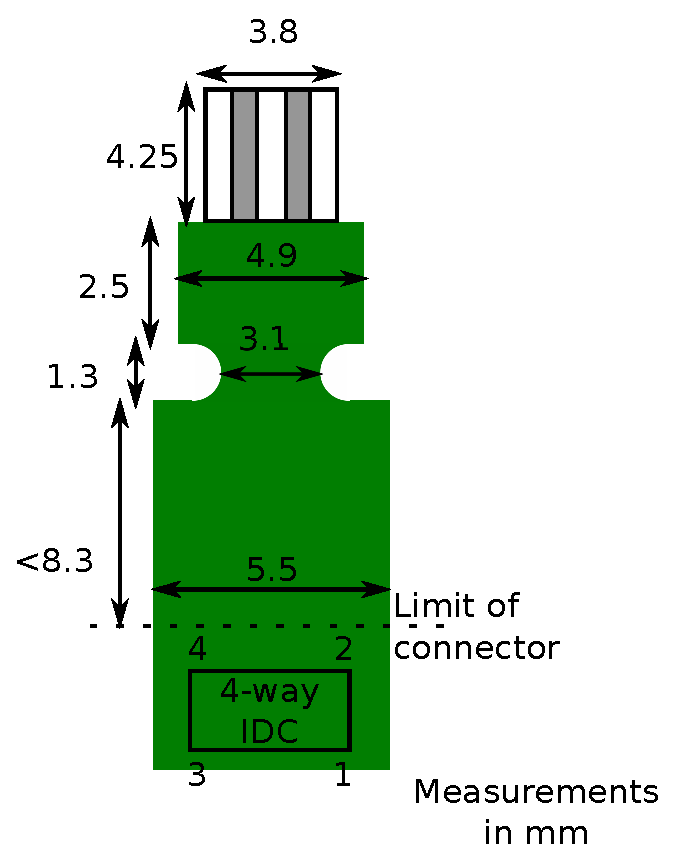
\includegraphics[width=0.4\textwidth]{imgs/sipmboardsize}
        \caption{Size of the SiPM board.}
        \label{fig:sipmboardsize}
    \end{center}
\end{figure}


\begin{table}[h]
    \begin{center}
        \caption{Pin mapping for the 4-way IDC socket on the SiPM board.}
        \label{tab:IDC4waySiPM}
        \begin{tabular}{cc}
            \hline
            \hline
            Pin & Function \\
            \hline
            1 & GND \\
            2 & GND \\
            3 & SiPM HV \\
            4 & SiPM LV \\
            \hline
            \hline
        \end{tabular}
    \end{center}
\end{table}

\begin{enumerate}
    \item \must{The SiPM board must fit within the existing 3D printed socket design, with dimensions as shown in \cref{fig:sipmboardsize}.}
    \item \must{The SiPM board must house a single S12752-050P SiPM.}
    \item \must{The SiPM board must connect to the SiPM ribbon cable using a 4-way 1.27 mm pitch IDC socket TE 7-188275-4 (Farnell 3784710).}
    \item \must{The 4-way IDE socket must be on the opposite side of the PCB to the SiPM.}
    \item \must{The socket pin connections must be as detailed in \cref{tab:IDC4waySiPM}, where pin 1 is closest to the polarisation pin of the connector. The matching connector on the ribbon cable will be TE 7-215083-4, (Farnell 149032).}
    \item \must{The cable used to connect to the SiPMs must be 1.27 mm pitch twist and flat ribbon cable, with coloured wires (such as 3M XXXX, Farnell XXXX).}
    \item \must{The PCB must be able to identify which specific SiPM sensor is soldered to it.}
    \item \should{The SiPM boards should be designed to ease the production of 3000 units.}
    \item \should{The PCB silkscreen should indicate which order the ribbon cable wires (either coloured or brown) correspond to the IDC socket.}
\end{enumerate}

\clearpage
\newpage
\subsection{In-detector sensor bus}

{\bf Designer: Wim Beaumont (and others?)}

An \I2C bus will be provided on a pair ribbon cables within each detector frame, to allow deployment of in-detector sensors.
Temperature and humidity sensors are expected to be deployed within the detector and other sensors or functionalities may be useful.
The sensor bus ribbon cables will connect to a dedicated sensor bus PCB attached to the covering plate on the detector frame.
This will be deployed below the two analog PCBs.
The 10-way ribbon cable will be split into two in-detector sensor buses.
On bus will have the \I2C and also two GPIO lines, the other will only have \I2C.
The sensor board interface PCB will be connected by a ribbon cable to the digital read-out board's \I2C buses.

\begin{enumerate}
    \item \must{The sensor interface PCB must connect to the two sensor ribbon cables using a 10-way IDC connector, 3M 4610-600 (Farnell 1758627) connector.}
    \item \must{The sensor interface PCB must connect to one 4-way and one 6-way sensor ribbon cable, each with a separate \I2C bus, as shown in \cref{tab:i2cbus}.}
    \item \must{The sensor interface PCB must be able to enable or disable power to the \I2C buses.}
\end{enumerate}

\begin{table}[h]
    \begin{center}
        \caption{Pin mapping for the 10-way IDC socket on the sensor board.}
        \label{tab:i2cbus}
        \begin{tabular}{cc|cc}
            \hline
            \hline
            \multicolumn{2}{c}{Bus 0} & \multicolumn{2}{c}{Bus 1}\\
            Pin & Function & Pin & Function \\
            \hline
            1 & 3.3 V & 7 & 3.3 V \\
            2 & SCL0 & 8 & SCL1 \\
            3 & SDA0 & 9 & SDA1 \\
            4 & GND & 10 & GND \\
            5 & NC / GPIO0? & & \\
            6 & NC / GPIO0? & & \\
            \hline
            \hline
        \end{tabular}
    \end{center}
\end{table}

The sensor boards themselves will potentially have multiple designs to meet the various needs.

\begin{enumerate}
    \item \must{The sensor board must connect to the sensor ribbon cable using either a 6-way 1.27 mm pitch IDC socket (TE 7-188275-6, Farnell 1056234) or a 4-way 1.277 mm IDC socket (TE 7-188275-4, Farnell 3784710).}
    \item \must{The socket pin connections must be as detailed in \cref{tab:indetectorpins}, where pin 1 is closest to the polarisation pin of the connector.}
    \item \must{Each sensor board should allow the selection of \I2C addresses per sensor.}
    \item \should{The cable used for the \I2C bus should be flat ribbon cable, visibly different from the twist and flat cable used for the SiPMs.}
\end{enumerate}

\begin{table}[h]
    \begin{center}
        \caption{Pin mapping for the 4-way and 6-way IDC sockets on the in-detector sensor boards.}
        \label{tab:indetectorpins}
        \begin{tabular}{cc|cc}
            \hline
            \hline
            \multicolumn{2}{c}{6-way bus} & \multicolumn{2}{c}{4-way bus}\\
            Pin & Function & Pin & Function \\
            \hline
            1 & 3.3 V & 1 & 3.3 V \\
            2 & SCL0 & 2 & SCL1 \\
            3 & SDA0 & 3 & SDA1 \\
            4 & GND & 4 & GND \\
            5 & NC / GPIO0? & & \\
            6 & NC / GPIO0? & & \\
            \hline
            \hline
        \end{tabular}
    \end{center}
\end{table}

\clearpage
\newpage
\subsection{Analog board}

{\bf Designer: Wim Beaumont}

The analog boards provide a programmable bias voltage to each SiPM and also amplify the signals from each SiPM.
Two analog boards will be used per detector plane.
All analog boards are identical.

\begin{figure}[h]
    \begin{center}
        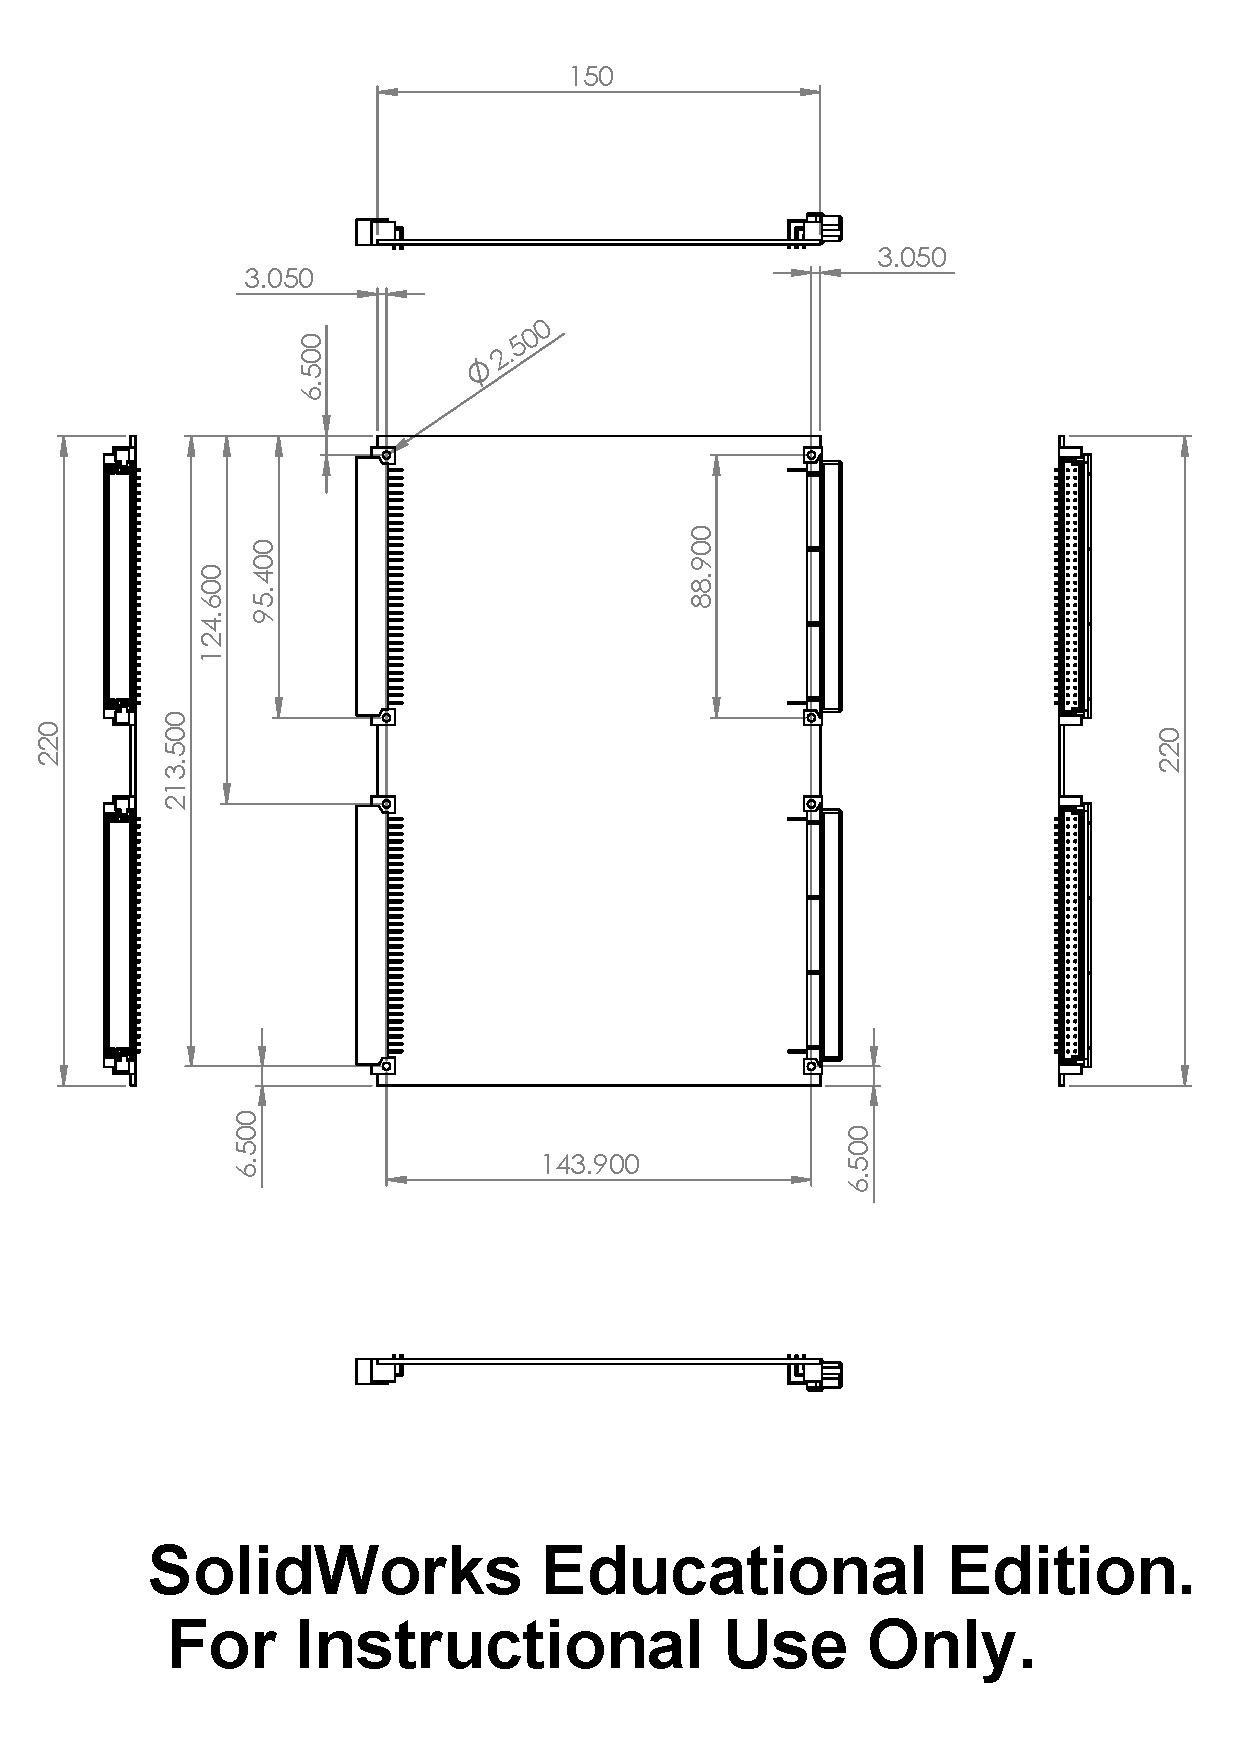
\includegraphics[width=0.8\textwidth]{imgs/Amplifier_Mod_2}
        \caption{Size of the analog board and positions of connectors.}
        \label{fig:analogboardsize}
    \end{center}
\end{figure}

\begin{figure}[h]
    \begin{center}
        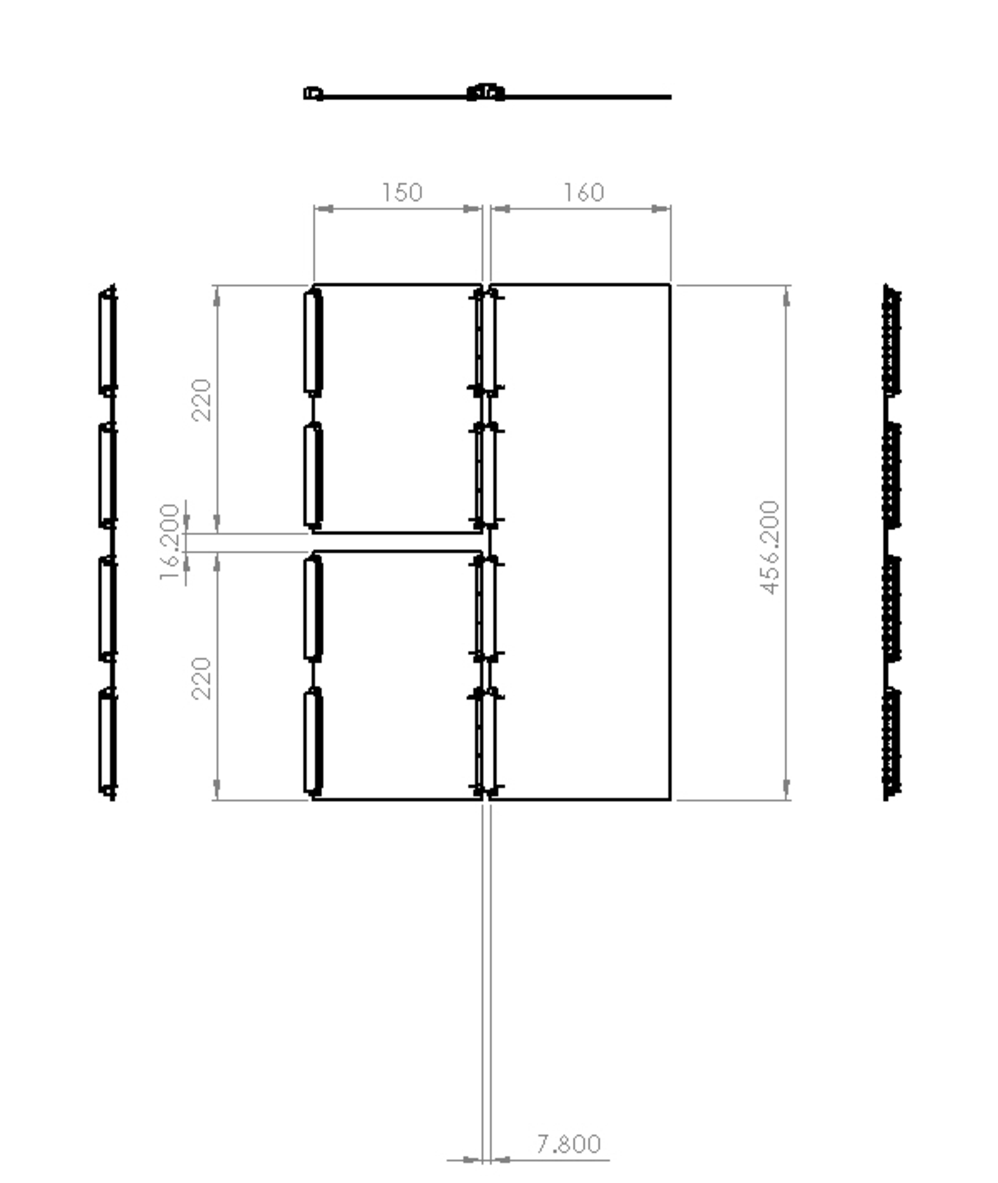
\includegraphics[width=0.8\textwidth]{imgs/Amplifier_Board_Pair_2D}
        \caption{Size and positions of both the analog and digital boards.}
        \label{fig:analogdigitalboardsize}
    \end{center}
\end{figure}

%\begin{figure}[h]
%    \begin{center}
%        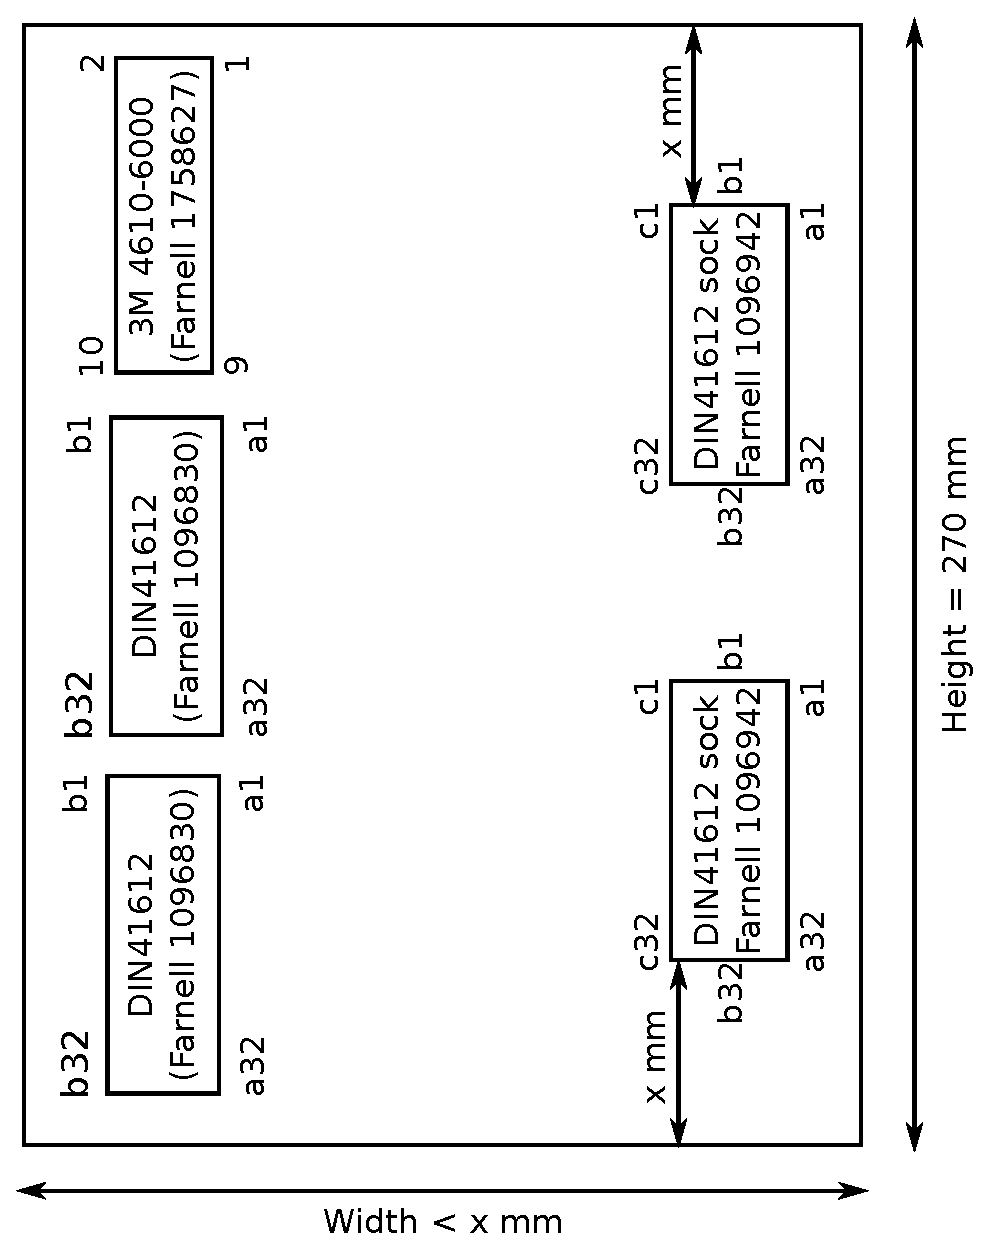
\includegraphics[width=0.8\textwidth]{imgs/analogboardsize}
%        \caption{Size of the analog board and positions of connectors.}
%        \label{fig:analogboardsize}
%    \end{center}
%\end{figure}

\begin{table}[h]
    \begin{center}
        \caption{Pin mapping for the lower 64-way DIN41612 socket housed on the analog board for connecting to the SiPM ribbon cable. The pin pattern is repeated 16 times. Note that pins A/B1 are towards the lower edge of the board.}
        \label{tab:lowerIDC64way}
        \begin{tabular}{cc|cc}
            \hline
            \hline
            Pin & Function & Pin & Function \\
            \hline
            A(1+2N) & SiPM$_N$ HV & A(2+2N) & GND \\
            B(1+2N) & SiPM$_N$ LV & B(2+2N) & GND \\
            \hline
            \hline
        \end{tabular}
    \end{center}
\end{table}

\begin{table}[h]
    \begin{center}
        \caption{Pin mapping for the upper 64-way DIN41612 socket housed on the analog board for connecting to the SiPM ribbon cable. The pin pattern is repeated 16 times. Note that pins A/B1 are towards the lower edge of the board.}
        \label{tab:upperIDC64way}
        \begin{tabular}{cc|cc}
            \hline
            \hline
            Pin & Function & Pin & Function \\
            \hline
            A(1+2N) & SiPM$_{N+16}$ HV & A(2+2N) & GND \\
            B(1+2N) & SiPM$_{N+16}$ LV & B(2+2N) & GND \\
            \hline
            \hline
        \end{tabular}
    \end{center}
\end{table}

\begin{table}[h]
    \begin{center}
        \caption{Pin mapping for the 3-way low-voltage power connector.}
        \label{tab:LVPower}
        \begin{tabular}{cc}
            \hline
            \hline
            Pin & Function \\
            \hline
            1 & +5 V \\
            2 & GND \\
            3 & -3.3 V \\
            \hline
            \hline
        \end{tabular}
    \end{center}
\end{table}

\begin{table}[h]
    \begin{center}
        \caption{Pin mapping for the 2-way high-voltage power connector.}
        \label{tab:HVPower}
        \begin{tabular}{cc}
            \hline
            \hline
            Pin & Function \\
            \hline
            1 & HV $\le 80 V$ \\
            2 & GND \\
            \hline
            \hline
        \end{tabular}
    \end{center}
\end{table}

%\begin{table}[h]
%    \begin{center}
%        \caption{Pin mapping for the 10-way IDC socket housed on the analog board for connecting to the in-detector I2C bus.}
%        \label{tab:IDC10way}
%        \begin{tabular}{cc|cc|cc|cc|cc}
%            \hline
%            \hline
%            Pin & Function & Pin & Function & Pin & Function & Pin & Function & Pin & Function \\
%            \hline
%            1 & GND & 3 & 3.3 V & 5 & NC & 7 & GND & 9 & 3.3 V \\
%            2 & SDA0 & 4 & SCL0 & 6 & NC & 8 & SDA1 & 10 & SDA1 \\
%            \hline
%            \hline
%        \end{tabular}
%    \end{center}
%\end{table}

\begin{table}[h]
    \begin{center}
        \caption{Pin mapping for the upper 96-way DIN socket connecting the analog to the digital board. Note that pins A/B/C1 are towards the lower edge of the board.}
        \label{tab:DIN96Upper}
        \begin{tabular}{cc|cc|cc}
            \hline
            \hline
            Pin & Function & Pin & Function & Pin & Function \\
            \hline
            A1 & GND & B1 & GND & C1 & GND \\
            A2 & A16+ & B2 & GND & C2 & A17+ \\
            A3 & A16- & B3 & GND & C3 & A17- \\
            A4 & GND & B4 & GND & C4 & GND \\
            A5 & A18+ & B5 & GND & C5 & A19+ \\
            A6 & A18- & B6 & GND & C6 & A19- \\
            A7 & GND & B7 & GND & C7 & GND \\
            A8 & A20+ & B8 & GND & C8 & A21+ \\
            A9 & A20- & B9 & GND & C9 & A21- \\
            A10 & GND & B10 & GND & C10 & GND \\
            A11 & A22+ & B11 & GND & C11 & A23+ \\
            A12 & A22- & B12 & GND & C12 & A23- \\
            A13 & GND & B13 & GND & C13 & GND \\
            A14 & A24+ & B14 & GND & C14 & A25+ \\
            A15 & A24- & B15 & GND & C15 & A25- \\
            A16 & GND & B16 & GND & C16 & GND \\
            A17 & A26+ & B17 & GND & C17 & A27+ \\
            A18 & A26- & B18 & GND & C18 & A27- \\
            A19 & GND & B19 & GND & C19 & GND \\
            A20 & A28+ & B20 & GND & C20 & A29+ \\
            A21 & A28- & B21 & GND & C21 & A29- \\
            A22 & GND & B22 & GND & C22 & GND \\
            A23 & A30+ & B23 & GND & C23 & A31+ \\
            A24 & A30- & B24 & GND & C24 & A31- \\
            A25 & GND & B25 & GND & C25 & GND \\
            A26 & GPIO2 & B26 & GND & C26 & GPIO3 \\
            A27 & +3.3 V & B27 & GND & C27 & +1.8 V \\
            A28 & GND & B28 & GND & C28 & GND \\
            A29 & SDA0 & B29 & GND & C29 & SCL0 \\
            A30 & GND & B30 & GND & C30 & GND \\
            A31 & GND & B31 & GND & C31 & GND \\
            A32 & +5 V & B32 & GND & C32 & +5 V \\
            \hline
            \hline
        \end{tabular}
    \end{center}
\end{table}

\begin{table}[h]
    \begin{center}
        \caption{Pin mapping for the lower 96-way DIN socket connecting the analog to the digital board. Note that pin A/B/C1 are towards the lower edge of the board.}
        \label{tab:DIN96Lower}
        \begin{tabular}{cc|cc|cc}
            \hline
            \hline
            Pin & Function & Pin & Function & Pin & Function \\
            \hline
            A1 & GND & B1 & GND & C1 & GND \\
            A2 & A0+ & B2 & GND & C2 & A1+ \\
            A3 & A0 & B3 & GND & C3 & A1- \\
            A4 & GND & B4 & GND & C4 & GND \\
            A5 & A2+ & B5 & GND & C5 & A3+ \\
            A6 & A2- & B6 & GND & C6 & A3- \\
            A7 & GND & B7 & GND & C7 & GND \\
            A8 & A4+ & B8 & GND & C8 & A5+ \\
            A9 & A4- & B9 & GND & C9 & A5- \\
            A10 & GND & B10 & GND & C10 & GND \\
            A11 & A6+ & B11 & GND & C11 & A7+ \\
            A12 & A6- & B12 & GND & C12 & A7- \\
            A13 & GND & B13 & GND & C13 & GND \\
            A14 & A8+ & B14 & GND & C14 & A9+ \\
            A15 & A8- & B15 & GND & C15 & A9- \\
            A16 & GND & B16 & GND & C16 & GND \\
            A17 & A10+ & B17 & GND & C17 & A11+ \\
            A18 & A10- & B18 & GND & C18 & A11- \\
            A19 & GND & B19 & GND & C19 & GND \\
            A20 & A12+ & B20 & GND & C20 & A13+ \\
            A21 & A12- & B21 & GND & C21 & A13- \\
            A22 & GND & B22 & GND & C22 & GND \\
            A23 & A14+ & B23 & GND & C23 & A15+ \\
            A24 & A14- & B24 & GND & C24 & A15- \\
            A25 & GND & B25 & GND & C25 & GND \\
            A26 & GPIO0 & B26 & GND & C26 & GPIO1 \\
            A27 & +3.3 V & B27 & GND & C27 & +1.8 V \\
            A28 & GND & B28 & GND & C28 & GND \\
            A29 & SDA1 & B29 & GND & C29 & SCL1 \\
            A30 & GND & B30 & GND & C30 & GND \\
            A31 & GND & B31 & GND & C31 & GND \\
            A32 & +5 V & B32 & GND & C32 & +5 V \\
            \hline
            \hline
        \end{tabular}
    \end{center}
\end{table}

\begin{enumerate}
    \item \must{The analog board height (as shown in \cref{fig:analogboardsize}) must be 220 mm.}
    \item \should{The analog board width should be 150 mm.}
    \item \must{The analog board must connect to two 16-SiPM ribbon cables via a 64-way 1.27mm pitch DIN41612 plug connector each (Farnell 1096830).}
    \item \must{The pin mapping for each IDC socket connectiong to the SiPM ribbon cables must be as described in \cref{tab:lowerIDC64way,tab:upperIDC64way}, with pin1 on the lower edge of the connector and row A {\bf on which side?}.}
    \item \must{The analog board must connect to the digital board using two 96-way DIN41612 socket connectors (Farnell 1096942).}
    \item \must{The pin mapping for the two connectors to the digital board must be as described in \cref{tab:DIN96Upper,tab:DIN96Lower}, with pins A/B/C1 on the lower edge of the connector and row A {\bf on which side?}}
    \item \must{The position of the two connectors to the digital board must be as shown in \cref{fig:analogboardsize}.}
    \item \must{The analog board must use input power connections of -3.1, GND, + 4.7 V (supplied by remote -3.3 V and +5 V power supplies), using a Molex 22-23-2031 connector (Farnell 1462950).}
    \item \must{The pin mapping for the low voltage connector must be as shown in \cref{tab:LVPower}, where pin 1 is defined as the left-most pin when the polarising shroud is upper-most.}
    \item \must{The analog board must regulate the input power to -2.8, GND, +4.4 V using linear regulators.}
    \item \must{The regulators must be controllable from the digital board to enable or disable powering the analog board components.}
    \item \must{The analog board must amplify the signal from each of 32 SiPMs using an AD8132 amplifier.}
    \item \should{The analog board should be compatible with replacing the DC connection to the digital board with an AC connection by replacing only passive components and not using the negative voltage power supply.}
    \item \must{The analog board must use high voltage input connections using a connector that is incompatible with the low voltage connector (perhaps JST VHR-2N (RS 820-1172).}
    \item \must{The pin mapping of the high voltage input must be as shown in \cref{fig:HVPower}, where pin 1 is defined as...}
    \item \must{A fuse must be used to protect the board from excessive current from the HV supply, to break at $I \le 100$ mA.}
    \item \should{The high- and low-voltage supply connectors should be clearly labelled on the PCB.}
    \item \must{The analog board must be able to produce a programmable high voltage bias supply on board, using ADL5317.}
    \item \must{The analog board must provide a per SiPM low voltage trim of up to 4 V using programmable DACs.}
    \item \must{The programmable DACs must be controllable by from the digital board via the \I2C buses on the two 96-way connectors.}
    \item \should{The channel numbering of the DACs should map simply to the channel numbering of the SiPMs.}
    \item \must{The analog board must provide an on-board temperature measurement and unique ID using an ATMEL AT30TSE752 chip with an \I2C address of 0b1001000 (i.e. all address pins connected to GND).} 
    \item \should{The temperature alert line from the temperature chip should be connected to one of the GPIO pins on the 96-way DIN connectors.}
\end{enumerate}

\clearpage
\newpage

\subsection{Digital board}

{\bf Designer: David Cussans}

The digital boards house an FPGA board which does front end processing and triggering.
They also digitise the amplified signals from the analog boards.
Each detector plane will use a single digital board, receiving data from two analog boards, as shown in \cref{fig:analogdigitalboardsize}.


%\begin{figure}[h]
%    \begin{center}
%        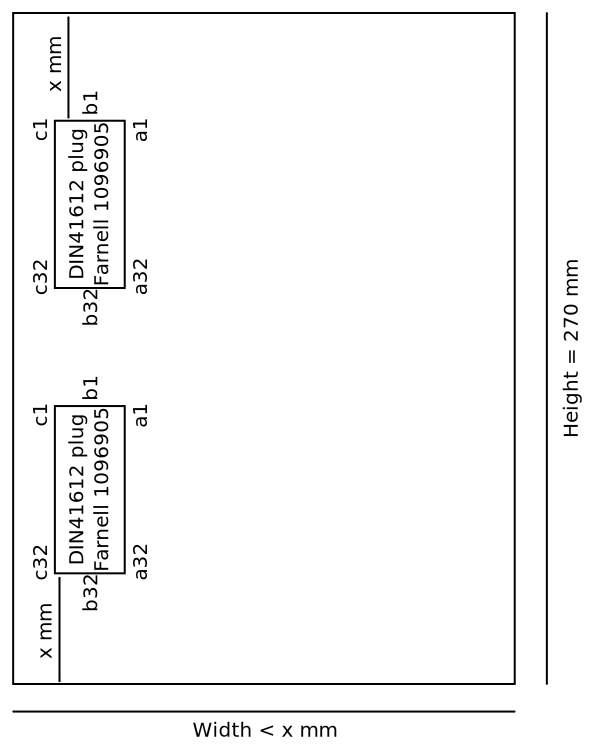
\includegraphics[width=0.8\textwidth]{imgs/digitalboardsize}
%        \caption{Size of the digital board and positions of connectors.}
%        \label{fig:digitalboardsize}
%    \end{center}
%\end{figure}


\begin{table}[h]
    \begin{center}
        \caption{LVDS pins available for ADC data on the Trenz 0712.}
        \label{tab:TrenzLVDS}
        \begin{tabular}{cccc}
            \hline
            \hline
            Connector & Bank & Pairs & \# Pairs \\
            \hline
            JM1 & 13 & 3, 5, 6, 9, 11 & 5 \\
            %JM1 & 16 & 16, 19, 17, 18, 9, 7, 11, 10, 5, 2, 6, 4, 1, 22, 24, 23, 15, 20, 21, 13, 14, 3, 12, 8 &  24 & 29 \\
            JM1 & 16 & 1-24 & 24 \\
            JM2 & 13 & 1, 2, 4, 10, 12-17 & 10 \\
            JM3 &  15 & 1-24 & 24 \\
            \hline
            \multicolumn{3}{c}{Total} & 63 \\
            \hline
            \hline
        \end{tabular}
    \end{center}
\end{table}

\begin{table}[h]
    \begin{center}
        \caption{Pin uses for Trenz 0712 bank 14 (3.3 V).}
        \label{tab:TrenzB14}
        \begin{tabular}{cc}
            \hline
            \hline
            Usage & \# pins \\
            \hline
            1 channel ADC data & 2 \\
            CPLD \I2C/SPI device select & 5 \\
            CPLD SPI (MOSI, MISO, CLK) or \I2C (SCL, SDAI, SDAO) & 3 \\
            %CPLD \I2C (SCL, SDAI, SDAO) & 3 \\
            Analog board GPIO & 8 \\
            LEDs & 4 \\
            IP address switches & 8 \\
            \hline
            Total & 30 / 30 \\
            \hline
            \hline
        \end{tabular}
    \end{center}
\end{table}

\begin{table}[h]
    \begin{center}
        \caption{Pin information for the HDMI connector used for the clock and synchronisation signals.}
        \label{tab:ClockSyncPins}
        \begin{tabular}{cc|cc|cc}
            \hline
            \hline
            Pin & Function & Pin & Function & Pin & Function \\
            \hline
            1 & SYNC+ & 2 & SYNC shield  & 3 & SYNC- \\
            4 & NC? & 5 & NC? & 6 & NC? \\
            7 & CLK+ & 8 & CLK shield & 9 & CLK- \\
            10 & NC? & 11 & NC? & 12 & NC? \\
            13 & Power Enable? & 14 & NC? & 15 & NC? \\
            16 & NC? & 17 & NC? & 18 & NC? \\
            19 & NC? & & & & \\
            \hline
            \hline
        \end{tabular}
    \end{center}
\end{table}

\begin{table}[h]
    \begin{center}
        \caption{Pin mapping for the connection between the digital board and \I2C interface board. {\bf To be defined...}}
        \label{tab:digitalToI2CInterface}
        \begin{tabular}{cc|cc}
            \hline
            \hline
            Pin & Function & Pin & Function \\
            \hline
            1 & ? & 6 & ? \\
            2 & ? & 7 & ? \\
            3 & ? & 8 & ? \\
            4 & ? & 9 & ? \\
            5 & ? & 10 & ? \\
            \hline
            \hline
        \end{tabular}
    \end{center}
\end{table}

\begin{enumerate}
    \item \should{The digital board height (as shown in \cref{fig:analogdigitalboardsize}) should be 466.2 mm.}
    \item \should{The digital board width should be 160 mm.}
    \item \must{The digital board must connect to the analog boards using two 96-way DIN41612 plug connectors (Farnell 1096905).}
    \item \must{The pin mapping for the connectors to the analog board must be as described in \cref{tab:DIN96Upper,tab:DIN96Lower}.}
    \item \must{The position of the two 96-way DIN41612 connectors must allow the analog boards' connectors to be be as shown in \cref{fig:analogboardsize}, with the spacing between the two analog boards as shown in \cref{fig:analogdigitalboardsize}.}
    \item \must{The digital board must allow a Trenz 0712 board to be plugged in.}
    \item \must{The pin usage/mapping for the Trenz board connections must be as shown in \cref{tab:TrenzLVDS,tab:TrenzB14}.}
    \item \must{The digital board must digitise 64 SiPM channels using 8 LTM9007 ADCs.}
    \item \must{The ADCs must be controlled via a 16-channel SPI-like bus, with two chip select lines per ADC chip.}
    \item \must{The digital board must have an HDMI connector to receive a clock and synchronisation signal, with the pin connection as shown in \cref{tab:ClockSyncPins}.}
    \item \must{The digital board must have an on board SiXXXX chip to clean the external clock signal and provide the clocks for the ADC chips and FPGA.}
    \item \must{The SiXXXX clock chip must be controlled by an \I2C bus on the digital board.}
    \item \must{The digital board must have an SFP+ cage for a Gbps Ethernet connection.}
    \item \must{The digital board must use input power connections of GND and 5 V.}
    \item \must{The digital board must convert the input power to 1.8 V and 3.3 V using on-board switching DC-DC converters.}
    \item \must{The DC-DC converters must be controllable from the FPGA, to enable/disable powering of the ADC.}
    \item \must{The powering of the FPGA should be controllable remotely via a control line on the HDMI clock/sync bus.}
    \item \must{The digital board should include a temperature sensor that can power down the FPGA if the board temperature exceeds a programmable alarm threshold.}
    \item \must{The digital board must have two eSATA sockets to allow Gbps serial communications between FPGAs from neighbouring planes.}
    \item \must{The digital board must have a 10-way IDC ribbon cable socket to connect to the in-detector sensor \I2C interface board.}
    \item \must{The connections to the \I2C interface board should be as defined in \cref{tab:digitalToI2CInterface}.}
\end{enumerate}

\clearpage
\newpage
\subsection{Clock distribution board}

{\bf Designer: David Cussans}

The clock distribution board provides the same clock to all digital boards.
In addition the board is able to provide a synchronous pulsed signal to all boards to ensure synchronisation across the detector.

\begin{enumerate}
    \item \must{The clock distribution board must provide a xxx MHz clock to all digital boards.}
    \item \must{The clock distribution board must provide a pulse signal synchronously to ten digital boards.}
    \item \must{It must be possible to enable or disable the synchronisation pulses from software.}
    \item \must{The clock and synchronisation signals must be provided via an HDMI connector.}
    \item \must{The HDMI connector pin mapping must be as shown in \cref{tab:ClockSyncPins}.}
    \item \must{The clock distribution system must have a hierarchical design. Each module of 10 detector planes should be served by a single clock distribution board, which in turn is served by a global 1:10 clock distribution board.}
    \item \should{The FPGA controlling the clock system should have a firmware tool chain compatible with the Artix-7 that will be used on the read-out board.}
\end{enumerate}

\clearpage
\newpage
\subsection{Power distribution board}

{\bf Designer: ?}

Power distribution boards should provide ten detector planes with the necessary high and low voltage power...

\clearpage
\newpage
\subsection{FPGA programming board}

{\bf Designer: Bristol electronics design group}

Each module of ten detector planes will have an FPGA programming board.
This will house a network accessible computer running the Xilinx programming software.
The board will fan out JTAG connections to each of the ten FPGAs in the detector module.


\clearpage
\newpage

\section{Review process}

The analog and digital schematics will be internally reviewed.
Following completion of the lay out for the two boards they will be reviewed by internal and external reviewers.
This review will have a larger scope, including the system level design of the read-out system.

\section{Time schedule}

This is the time schedule discussed at the collaboration meeting at Imperial in May 2016.
It is based around designing and reviewing the design before producing sufficient electronics to instrument 5 detector planes.
These will then be tested and validated before starting a larger production for 50 planes.

\begin{figure}[h]
    \begin{center}
        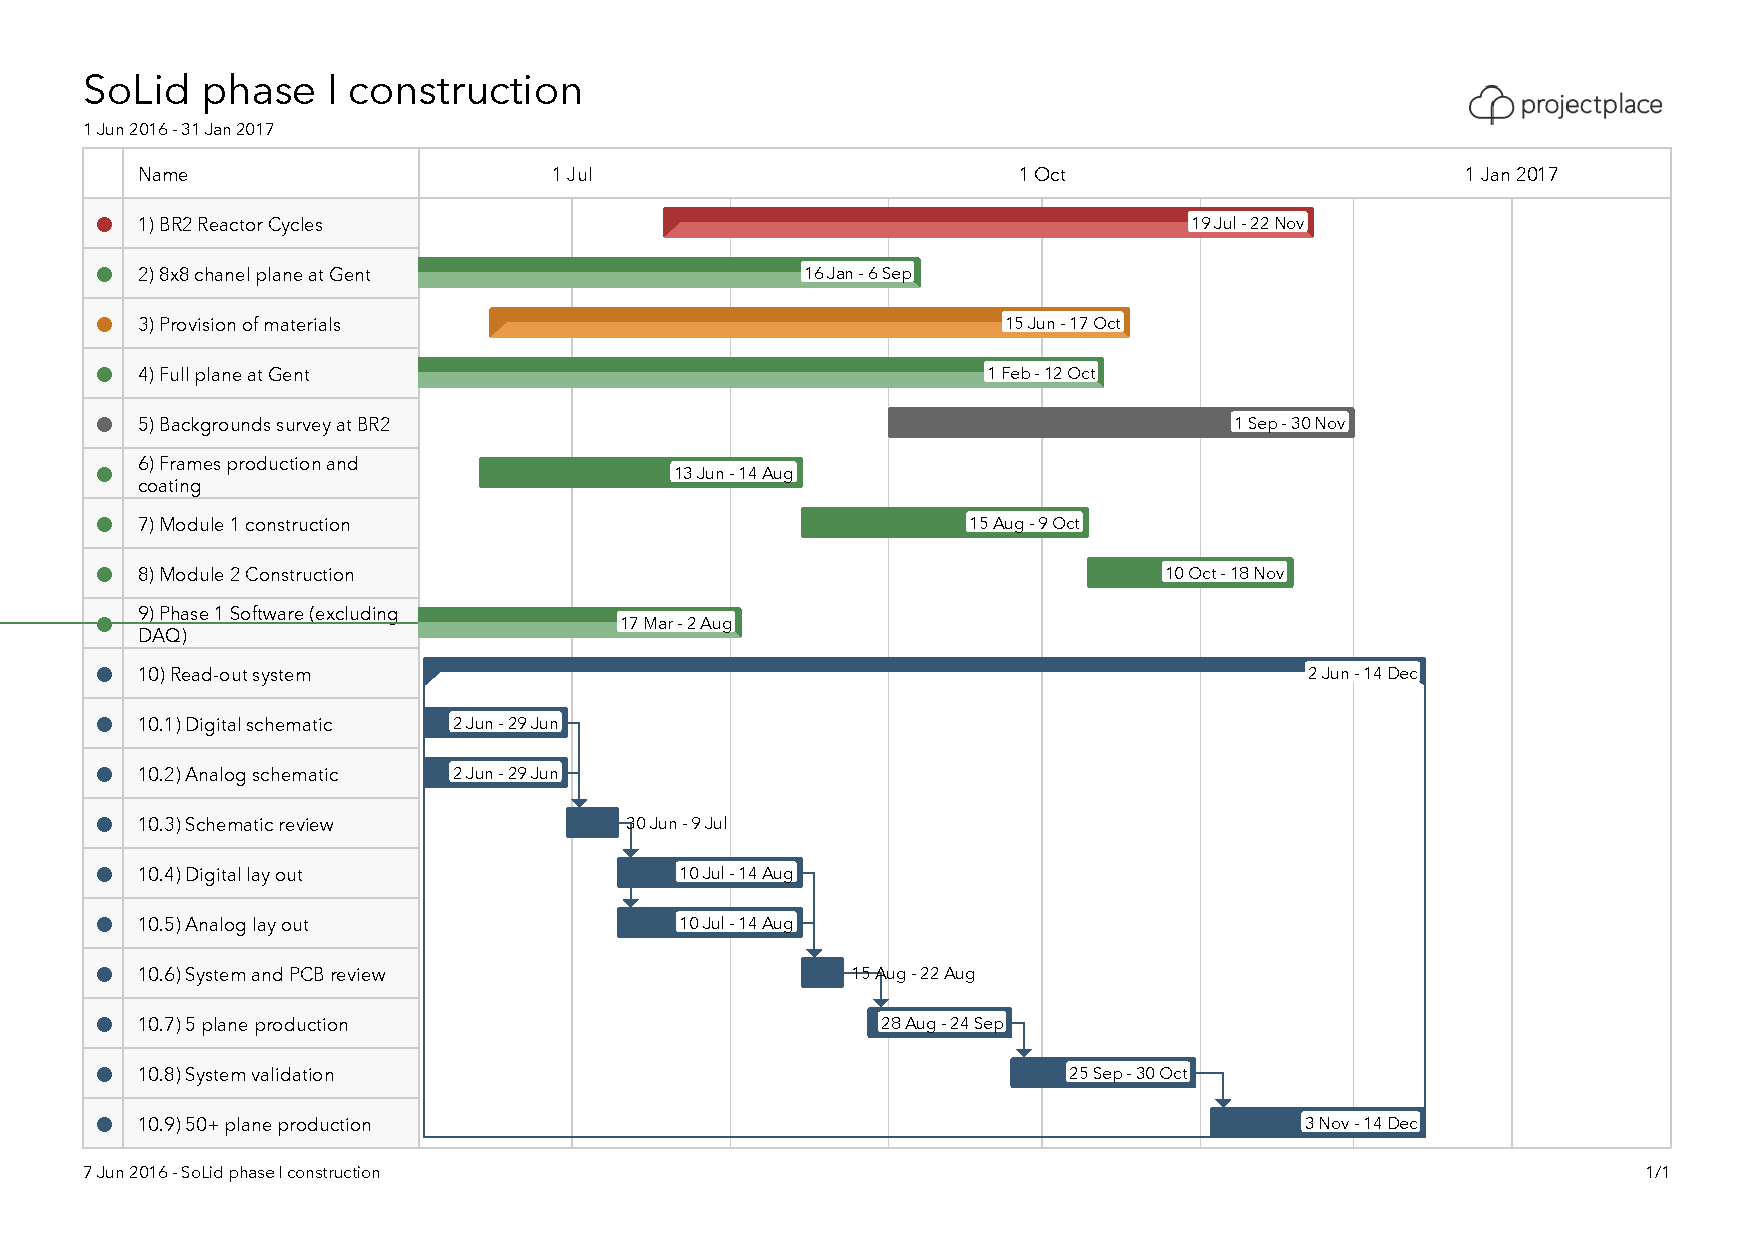
\includegraphics[width=0.95\textwidth]{imgs/Gantt}
        \caption{Estimated schedule, where task 10 corresponds to the electronics described in this specification.}
        \label{fig:gantt}
    \end{center}
\end{figure}


\end{document}
